\documentclass[a4paper, 12pt, oneside]{book}
\usepackage[a4paper, left=2.5cm, right=2.5cm, top=3cm, bottom=3cm]{geometry}
\usepackage{times}
\usepackage{url}
\usepackage{graphicx}
\usepackage{textcomp}
\usepackage{xcolor}
\usepackage{xspace}
\usepackage{float} 
\usepackage[nottoc, notlot, notlof, notindex]{tocbibind}
\usepackage{latexsym}
\usepackage{amsmath,amssymb,amsfonts}
\usepackage{algorithm}
\usepackage[noend]{algpseudocode}
\usepackage{setspace}
\usepackage{rotating}
\usepackage{footnote}

\newcommand{\subsubsubsection}[1]{\paragraph{#1}\mbox{}\\}
\setcounter{secnumdepth}{4}
\setcounter{tocdepth}{4}

\usepackage{listings}
\usepackage{hhline}
\lstset
{ %Formatting for code in appendix
	basicstyle=\fontsize{9}{11}\ttfamily,
	escapeinside={<@}{@>},
	showstringspaces=false,
	tabsize=1,
	breaklines=true,
	breakatwhitespace=false
}
\usepackage{colortbl}
	\definecolor{Gray}{gray}{0.9}
\usepackage{color}
\usepackage{tcolorbox}
\tcbuselibrary{listingsutf8}
\usepackage{enumerate}
\usepackage{tabularx,adjustbox,booktabs}
\usepackage{array}
\usepackage{tcolorbox}

\newcommand\setrow[1]{\gdef\rowmac{#1}#1\ignorespaces}
\newcommand\clearrow{\global\let\rowmac\relax}
\clearrow

\def\BibTeX{{\rm B\kern-.05em{\sc i\kern-.025em b}\kern-.08em
		T\kern-.1667em\lower.7ex\hbox{E}\kern-.125emX}}


\title{Why can't we build all commits of the history of a project? An empirical study}
\author{Michel Maes Bermejo}

\renewcommand{\baselinestretch}{1.5}

\begin{document}

%%%%%%%%%%%%%%%%%%%%%%%%%%%%%%%%%%%%%%%%%%%%%%%%%%%%%%%%%%%%%%%%%%%%%%%%%%%%%%%%
% PORTADA
\cleardoublepage
\begin{titlepage}
\begin{center}
\begin{tabular}[c]{c c}

\includegraphics[scale=0.6]{img/urjc-logo.jpg} &
\end{tabular}

\vspace{1cm}

\Large
MASTER EN SISTEMAS DE INFORMACI\'{O}N

\vspace{0.4cm}

\large
Curso Acad\'{e}mico 2018/2019

\vspace{0.8cm}

Trabajo Fin de Master

\vspace{2cm}

\LARGE
Why can't we build all commits of the history of a project? An empirical study

\vspace{2cm}

\large
Autor : Michel Maes Bermejo \\
Tutor : Micael Gallego Carrillo

\end{center}
\end{titlepage}

%%%%%%%%%%%%%%%%%%%%
%%%% Resumen
%%%%%%%%%%%%%%%%%%%%

\chapter*{Abstract}
\pagenumbering{gobble}

%Context: 
The buildability of a software project is the ability to build it from its sources. 
Buildability has been usually studied only in stable points of its history (in general, its releases / versions).
But it may be also useful to study buildability for all past snapshots (i.e., all past states of the system after a commit) of a project, for instance for a security audit or to search for bugs.
%Goal:
In this work we analyze the buildability of all snapshots of six open source projects, and categorize the problems that occur during this process and that make the software projects be not-buildable.
%Method:
For this we try to build all past snapshots of the projects under study, analyze how many of them we are able to build and record the output if the build process fails.
Based on an analysis of the failing builds, we propose a taxonomy of failures.
%Results:
In average, more than 50\% of the snapshots of the projects under study are not buildable.
The main problem we find (80\% of fails) is related to the change of technology in the build system in the history of the project, followed by semantic problems (8\%) and dependency problems (7\%).
%Conclusion:
Analyzing the root causes of failing snapshots, we estimate that using the correct build system along the history, we could reduce the number of not-buildable snapshots from 50\% to 17\% of the total.




%%%%%%%%%%%%%%%%%%%%
% �NDICES %
%%%%%%%%%%%%%%%%%%%%

%%%% �ndice de contenidos
\tableofcontents 
%%%% �ndice de figuras
\cleardoublepage


%%%%%%%%%%%%%%%%%%%%%%%%%%%%%%%%%%%%%%%%%%%%%%%
%       1.INTRODUCCI�N Y MOTIVACI�N           %
%%%%%%%%%%%%%%%%%%%%%%%%%%%%%%%%%%%%%%%%%%%%%%%

\chapter{Introducction}
\label{sec:intro} 
\pagenumbering{arabic}
%This research started as a \emph{side effect} of another investigation that we were carrying out.

To find out whether regression tests, created when a bug is fixed in a project, could help to analyze the \emph{origin} of that bug, we intended to run the test on past versions of the software.
The snapshot (commit) where the test fails would be the candidate for being the bug-introducing change~\cite{kim2006automatic}.
To do this, it was necessary to first build and then run the regression test on the previous snapshots of the project.
We found, however, that many of the snapshots were not buildable.

The dataset we used was the same as the one we were going to do in this study, Defects4J~\cite{Just:2014:DDE:2610384.2628055}.
Exploring other investigations that made use of this same dataset, we identified another study that had the same problems trying to build some snapshots~\cite{Just:2014:MVS:2635868.2635929}.
The authors decided to discard from their study those that did not build.
We discovered that in some cases it was possible to fix some of the build failures.
However, the diversity of errors motivated us to make a deeper analysis in the different projects, studying how buildable the snapshots were, and to create a taxonomy to understand and classify the most recurrent errors.

We are not the only ones interested in such an endeavor.
Both industrial software developers and software engineering researchers have shown interest in rebuilding past snapshots of projects~\cite{nikitin2017chainiac, RepBlds:2017:Online}, and do it in their day-to-day work.
Rebuilding the past snapshots of a software project is done with different objectives in mind, among others:

\begin{itemize}
	\item \textbf{{To search and find bugs}}: In line with our original intention, software developers often run previous snapshots of the system in order to localize bugs and understand how they originated~\cite{Zimmermann:2006:MVA:1137983.1138001}.
	\item \textbf{{Due to security reasons}}: Users usually trust the available binaries of a library, but a backdoor could be inserted~\cite{deCarnedeCarnavalet:2014:CIV:2664243.2664288}.
Rebuilding a library version from the original source allows to compare the binaries to verify that no new code has been introduced.
	\item \textbf{{To backport bug fixes}}: To apply a patch or an update to an older version of the software, it is necessary to be able to build that specific version~\cite{tian2017mining}.
	\item \textbf{{To reproduce the past state of a system}}: For research, it is often useful to obtain a functional binary/executable to verify the correct performance of the system~\cite{manacero2011using}.
	The use of the project history is also useful to predict future bugs~\cite{Zimmermann2008}.
\end{itemize}

%\grex{I don't understand why we put the `desirable features' here... this is something very specific that belongs to the method section or when we are presenting the case studies.}


% In the literature, build reproducibility is the ability to generate byte-to-byte identical binaries from the source code of the project, at any point of its history, no matter who builds the binary, when or in which machine~\cite{RepBldsDebian:2018:Online}.

Sulir and Porub\"an~\cite{Sulir:2016:QSJ:3001878.3001882} consider, in the context of projects created with compilable languages, the build process to be composed of the following steps:

\begin{enumerate}
	\item read the project build file
	\item download third party components defined in the build file
	\item execute the compiler to generate  binary files from source code, and
	\item package the program in a suitable format for deployment.
\end{enumerate}

For them, a specific project version is {\bf buildable} if these steps can be executed to generate a valid binary.
A related term is {\bf build reproducibility}, which is \emph{the ability to generate byte-to-byte identical binaries from the source code of a project version, no matter who builds the binary, when or in which machine}~\cite{RepBldsDebian:2018:Online}.
Reproducible builds create thus a verifiable path from human readable source code to the binary code used by computers, and are gaining relevance in recent times~\cite{cito2017empirical, maudoux2018correct}, in particular, but not limited, in relation to Blockchain technologies~\cite{deCarnedeCarnavalet:2014:CIV:2664243.2664288, perry2014reproducible}.
It should be noted that to generate a reproducible build from a specific version of a project, first that version should be buildable, and then additional conditions have to be met.
Build reproducibility may be pursued when security is a key characteristic, but there are many scenarios --as those pointed out above-- where having \emph{just} buildability should be \emph{enough}.

We define the {\bf buildability of a project} as \emph{the ability to build a project from its sources}.
Buildability is essential for any software project, as it has to be run.
In this work, we argue that buildability should not be limited to the current (i.e., latest) version of a software, but to all its history (or at least part of it) -- we refer to this ability as {\bf historic buildability}, and in particular to {\bf complete historic buildability} when \emph{all past versions of a software project can be built}.

Ideally, a version successfully built in the past should be built successfully nowadays.
However, the evolving nature of software has as a (non-intended) consequence that this is not always the case.
We have studied the buildability of the history of several projects checking if their snapshots are buildable or not.
We have focused on six well-known open source Java projects.
Five are taken from the Defects4J repository~\cite{Just:2014:DDE:2610384.2628055}, commonly used in Software Engineering research.
The other one is the Spring Framework project~\cite{Spring:2019:Online}, a big open source project commonly used in the industry for building web applications.
Specifically, this work tries to answer following research questions:

\begin{itemize}
	\item \textbf{RQ1}: Can we build all snapshots of a project? 
    This research question will shed some light into how \emph{historic buildable} software projects are. We consider a build as successful if a snapshot is buildable, and a fail if not.
	\item \textbf{RQ2}:  What are the most common problems that cause snapshot build fail?
    In addition to determine what problems prevent snapshots to be buildable, we propose a classification of the problems into different categories.
\end{itemize}

The contributions of this paper are following:
    
\begin{enumerate}
	\item To the best of our knowledge, this is the first work to address the buildability of all the snapshots of a project.
	\item We propose simple and generic tools to check the buildability of a project's history, and analyze the problems that make a snapshot build fail.
	\item We propose a taxonomy of build failures with an empirical base.
	\item We provide the extension of a previous dataset~\cite{Just:2014:DDE:2610384.2628055} including the history of buildable snapshots and the logs in the case in which they were not buildable for the projects studied.
\end{enumerate}

The work is structured as follows:
Previous work is presented in Section~\ref{sec:related}.
Subject project, tools and methodology is presented in Section~\ref{sec:metodology}.
Section~\ref{sec:results} and Section~\ref{sec:taxonomy} answer the research questions.
In Section~\ref{sec:discussion} we discuss about the work carried in this work.
Finally, Section~\ref{sec:conclusions} concludes the work.
 

\chapter{Related work}
\label{sec:related}
Probably the most relevant research on build errors is the empirical study by Seo et al.~\cite{Seo:2014:PBE:2568225.2568255} that examined over 26.6 million builds triggered in Google's centralized build environment.
An error taxonomy was provided by this study based on log patterns.
%\grex{What differs or adds our work in comparison to this one?}
Sulir and Porub\"an examine the builds of more than 7000 Java projects, but only for their last commit~\cite{Sulir:2016:QSJ:3001878.3001882}.
In both studies, they have performed a study \emph{in amplitude}.
Compared to them, in this this work, we will limit the number of projects to study all their history -- our effort can thus be considered a study in depth.

Rausch et al.~\cite{Rausch:2017:EAB:3104188.3104231} address the reasons why builds fail in the context of Continuous Integration (CI) environments.
These authors extracted outputs from Travis (a CI tool) from 14 open-source projects, along with information from their public Git repositories.
An important percentage of error outputs correspond to the tests that have not passed, but they give special importance to the cases where the failed build previous to the tests is the cause of the error.
In addition to categorize the main errors found by the CI system, they also consider other metrics (e.g., number of authors, number of lines modified, frequency of changes, among others).
The study contemplates the analysis of the history of the builds from the approach of continuous integration (construction of the project together with the tests).
Our approach tries to verify what would happen if instead of taking the outputs of CI, we execute ourselves the build of the project (not considering tests) to check if all commits are able to be built (i.e., if the commit is buildable).
Rausch et al.'s study is limited to the builds made by the CI, which do not correspond to the number of commits of the project.
%It is therefore a line to approach to check if all the commits of a project can be built.

Buildability may have a huge impact on those areas where building past commits of the project is key.
This is the case for bug localization~\cite{Sliwerski:2005:CIF:1083142.1083147,Asaduzzaman:2012:BIC:2664446.2664463, Murgia:2010:MLA:1852786.1852794, Zimmermann:2006:MVA:1137983.1138001, Zimmermann2008}.
When localizing bugs, techniques like git bisect may be used to traverse the project history of commits back to the past in order to find the set of lines in a commit that introduced a bug~\cite{spinellis2012git, meneely2013patch}.

Some authors have emphasized the importance of historical versions to propose repair tools of failed builds~\cite{HireBuild}, or have proposed metrics to evaluate the stability of the project over time~\cite{6405296}.
Others have addressed the problem in an indirect way.
For instance, Just et al. found this problem when trying to run mutant tests in previous versions of several software projects~\cite{Just:2014:MVS:2635868.2635929} provided by Defects4J~\cite{Just:2014:DDE:2610384.2628055}.

Reproducibility of research is a popular topic of interest among researchers to validate findings from other publications~\cite{RODRIGUEZPEREZ2018164} and projects~\cite{4693714}.
Although much attention has been put on the availability of publicly available datasets (e.g., datasets on defect prediction~\cite{wahono2015systematic}), the software developed and used by researchers has shown to have major importance~\cite{rodriguez2012software, bruntink2014initial}.
The software engineering research community has proposed some solutions that facilitate scientific software reproducibility in the future~\cite{DBLP:journals/corr/Weber17,DockerReproducibility2016,Boettiger:2015:IDR:2723872.2723882}.

%The reproducibility of experiments in software engineering is a subject widely discussed by Juristo et al.~\cite{juristo2004improving,juristo2011role,gomez2014understanding}.


%\grex{We have to mention Juristo's work in empirical software engineering on reproducing experiments}

%Gonz{\'a}lez-Barahona and Robles note that ``reproducibility of experiments is one of the basic rules in the scientific method''~\cite{González-Barahona2012}.


As pointed out in the introduction, a term related to buildability and very recurrent recently is build reproducibility.
%buildability is the first step to achieve reproducibility and therefore the focus of our research.
%Build reproducibility is the ability to generate byte-to-byte identical binaries from the source code of the project, at any point of its history, no matter who builds the binary, when or in which machine~\cite{RepBldsDebian:2018:Online}.
%Some authors also include test in build process.
Software distributors, such as the Debian community, have a strong interest in the reproducibility of builds~\cite{RepBlds:2017:Online,RepBldsDebian:2018:Online}.
Ren et al. focus on reproducible builds in Debian packages~\cite{Ren:2018:ALU:3180155.3180224}.
In it, the authors present a framework for detecting and fixing reproducible problems in Debian packages, but they focus exclusively on the latest commit, and they do not analyze the reproducibility of those packages in the past.
Glukhova also discusses the reproducibility of Debian packages by offering tools that ensure reproducibility~\cite{Glukhova:Thesis:2017}.
The reproducibility of builds is also interesting from a security point of view.
Some works focus on bringing security into the software development life cycle, and they mention build reproducibility as one of the main issues to be taken into account.
De Carn\'e de Carnavalet and Mannan mention the use of reproducible builds in the context of security-critical open source software~\cite{deCarnedeCarnavalet:2014:CIV:2664243.2664288}.
Nikitin et al. propose a decentralized software-update framework that includes build verifiers to validate the source-to-binary correspondence~\cite{nikitin2017chainiac}.
Al-Bassam and Meiklejohn propose a system to ensure binary transparency~\cite{10.1007/978-3-030-00305-0_8}.
Skrimstad noted about the trust in software through reproducible builds~\cite{Skrimstad:Thesis:2018}.

Build reproducibility is typically studied in stable versions of the project where a binary is available.
We are interested in building not only the stable versions, but all project snapshots for which there is usually not binary, which allows to be used in scenarios such as bug fixing, among others.
Thus, while a software project requires to meet additional criteria to achieve build reproducibility than to be buildable, complete historic buildability demands a software project to have many more snapshots to be buildable.

%In comparison, our work addresses all versions (releases, betas and snapshots), instead of just the latest stable version.

%\grex{You say there is just one work, but then refer to two}

%\grex{A good idea here would be to tell how our approach differs from what has been previously done.}





\chapter{Methodology}
\label{sec:metodology}
Our objective is to analyze multiple projects, checking whether we can build  or not every snapshot.
For those snapshots whose build fails, we study the build logs to determine which are the most common errors that prevent a snapshot from being buildable, grouping and categorizing errors in a taxonomy.

%Reproducibility is a topic of interest among researchers to validate other publications~\cite{RODRIGUEZPEREZ2018164} and projects~\cite{4693714} through reproducibility, in addition to offering solutions that facilitate reproducibility in the future~\cite{DBLP:journals/corr/Weber17,DockerReproducibility2016,Boettiger:2015:IDR:2723872.2723882}. For this reason,
 
We have tried to make our experiment reproducible so that any researcher can obtain the same results as we do or use our data for other investigations.
The reproducibility package for this work can be found in a public repository, that has been anonymized to comply with the double blind review process\footnote{https://github.com/AnonymusDeveloper2019/PastBuilds}.

%\mica{New section to discuss reproducibility of the project?}
%\grex{This belongs to the methodology section and should be better a footnote with the URL, not a cite.}

\section{Subject programs}

To choose what projects are suitable for this study, we consider some desirable characteristics that make them easy to build:

\begin{itemize}
	\item Using a compiled language (e.g., Java or C++), so that when developing, type-safety is enforced during the build phase, avoiding type problems in runtime.
In addition, we can obtain more information at the build phase than from projects using a dynamic language.
	\item Project dependencies are simple to obtain, for example, from a remote repository.
	\item The environment in which the project was built is easy to set up, or has no impact on the build.
\end{itemize}

Following Easterbrook \emph{et al.}~\cite{easterbrook2008selecting}, we selected six exploratory case studies to gain a deep understanding of the buildability in six open source projects.
For this purpose, we selected projects written in Java, a static typed programming language that is platform-independent, with a freely available compiler.
Java has also backward compatibility and multiple tools to manage dependencies like Maven, Gradle or Ant.
In order to study the buildability of a project, the history of the projects needs to be available through some source control management (SCM) system.
The selected projects are available in git repositories, so we used git to traverse their history.

Table~\ref{table:projects} shows the six open source Java projects selected for the study.
For each project, we display the number of snapshots (commits) that are available in their respective git repositories, and the build system used by the project to compile the source code and generate the binaries.
Five projects come from a common dataset in software research, Defects4J~\cite{Just:2014:DDE:2610384.2628055}.
These projects are commonly used for research in Software Testing.
It is important to note that they are small projects with a limited set of dependencies\ref{table:projects}.
The only exception is the Closure project, with 12 dependencies, which are included in the source code without the need to recover them from an external repository.

%\grex{Could we have the number of dependencies as well? As I suppose they vary over time, it would be good to provide a range of the number of dependencies.}
To expand our dataset, we also analyze the Spring Framework project.
This project is a large multi-module project, widely used in the industry for developing Java web applications.
The complexity of this project is far beyond that of the Defects4J projects.
It has as well a higher number of dependencies.

\begin{savenotes}
	\begin{table}
		\caption{Projects used in this work}
		\label{table:projects}
		\centering
		\begin{tabular}{crcr}
			\toprule
			\bf{Project} & \bf{\# Snapshots} & \bf{{Build system}} & \bf{\# Dependencies}\\ 
			\midrule
			Closure Compiler & 2,858 & Ant & 12\footnote{Dependencies are in source files}\\
			Commons-lang & 3,570 & Maven & 3\\
			Commons-math & 4,878 & Maven & 1\\
			Mockito & 2,639 & Gradle & 4\\
			Joda-Time & 1,717 & Maven & 2\\
			Spring Framework & 17,382 & Gradle & 20\footnote{Optional dependencies are not counted}\\
			\bottomrule
		\end{tabular}
	
	\end{table}
\end{savenotes}

\section{Analysis process}

The analysis consisted in two phases, a first one for checking buildability of the project (\textit{Check build process}), and a second one for analyzing the data collected of the failed builds (\textit{Log analysis}) in order to perform the classification.

%\grex{I don't know if ``experiment'' is the right wording}

\subsection{Check build process}

This process is shown in Figure~\ref{fig:commitHist}.
It starts with the most recent commit of the project.
This commit is checked out, and the project is built from its source files using the appropriate build system for the project (as defined in Table~\ref{table:projects}).
To determine the build status, we check the exit code of the build process: zero signifies success, and non-zero signifies failure.
If the build succeeds, it is marked as success.
Otherwise, it is marked as failure and the logs generated during the build process are saved for later inspection.
Then we go back to the previous commit, and repeat the whole process.
This process is repeated until we reach the first commit in the repository.
Figure~\ref{fig:commitHist} summarizes the process in a visual form.

\begin{figure}[h]
	\centering    
	\includegraphics[width=12cm]{img/CommitHist.pdf}
	\caption{Check build process}
	\label{fig:commitHist}
\end{figure}

Due to the large number of commits in the history of the selected projects, building them manually is not practical.
In order to automate the process, we developed a Python script that given a configuration file, a build script and the git project, basically executes the process described above iteratively for each commit.
To build each project, the basic commands of each construction tool have been used, taking into account the documentation of each project (e.g., a Maven build is shown in Listing~\ref{listing:mvnscrpt}).
In most projects, it is important to clean the output folders to avoid reusing files when changing between commits.
To reproduce these steps in a simple way without having to worry about the environment or the necessary technologies, this execution is encapsulated in a Docker\footnote{https://www.docker.com} container.

%\mica{Ampliar esto mencionando que incluye este paquete}

%\grex{I would like to hear something about the dependencies here...I remember hearing from Michel that he set up an environment where he run the experiment... please, include that info here!}

\begin{lstlisting}[caption={Example of a Maven build command},captionpos=b, label={listing:mvnscrpt}]
                      mvn clean install -Dmaven.test.skip=true
\end{lstlisting}


\subsection{Log analysis} 
\label{sssec:logAnalysis}

Our analysis (depicted in Figure~\ref{fig:AnalysisProcess}) takes as input:
   i) the commit history of the project (where each commit is marked as success or failure), and
   ii) the logs for the commits marked as a failure.
Our aim is to perform an analysis of the logs to determine the reasons why the build failed.

\begin{figure}[h]
	\centering    
	\includegraphics[width=12cm]{img/AnalysisProcess.pdf}
	\caption{Analysis process for builds that fail.}
	\label{fig:AnalysisProcess}
\end{figure}

We assume that consecutive commits which fail between two successful commits are likely to contain the same error.
Based on this idea, choosing a log from a group of consecutive commits, we can extract the error trace that identifies the problem and generate a pattern from it.
Once we have a consistent number of patterns, we apply them in order (from more specific to more generic) to each log, stopping when a match occurs, continuing with the next log.
This process is iterative: new patterns are generated to eliminate very generic patterns and group the logs better.
We finish the process when all logs match a pattern and can be grouped without confusion.

We will call this error trace a \textbf{symptom}.
We then group similar patterns together, in order to identify those logs that share the same symptom.
For each symptom that we find, a \textbf{cause} (i.e., the error that causes the symptom) can potentially be attributed to it.
The cause, in many cases and due to the Java logging system, can be extracted together with the symptom.
In other cases, the cause is more ambiguous and requires interpreting the log along with the failed version of the project, exploring it in detail (sometimes at a very low-level).
In the most difficult cases, the authors met to review and discuss until they reached an agreement.
In a next step, our intention is to categorize the error according to its nature using a method for taxonomy development.

%Once the cause is determined, we assess \textbf{if the error could be solved} by applying a change -- or if it is unsolvable.
%In case it is solvable, it is necessary to determine if it needs a) a simple change (e.g., adding a trivial script during the build) or b) a major change is necessary (e.g., a non-trivial modification of the source code).
%\michel{We should mantain this? We have no solutions for the errors}

To clarify the process, we present a didactic example is shown in Listing~\ref{listing:pattern}.
In this case, an error pattern is applied to the log obtained after a failed execution in the Spring Framework.

% \textcolor{black}{Pattern: }
\begin{center}
	\begin{lstlisting}[linewidth=\linewidth, caption={SpringFramework Log - Commit 8961}, captionpos=b, label={listing:pattern}]
	<@\textbf{Pattern: }@><@\textbf{\textcolor{violet}{Could not find (.+)}}@>m
	<@\textbf{Log with pattern matching: }@>
	FAILURE: Build failed with an exception.
	
	* What went wrong:
	Could not resolve all dependencies for configuration ':spring-messaging:optional'.
	> <@\textbf{\textcolor{violet}{Could not find org.projectreactor:reactor-net:1.1.0.BUILD-SNAPSHOT.}}@>
	Required by:
	org.springframework:spring-messaging:4.1.0.BUILD-SNAPSHOT
	\end{lstlisting}
\end{center}


\begin{itemize}
	\item \textbf{{Symptom}}: The trace highlighted in the log can not resolve a dependency.
	\item \textbf{{Cause}}: An unspecified development (BUILD-SNAPSHOT) version is used and can not be recovered.
	%\item \textbf{{Could be solved?}}: It is resolvable, apparently easy, replacing the version with a stable one (release)
\end{itemize}



%\grex{I think it would be very didactic to show an example of an error log, to highlight where we see that we can find the cause. Doing this with an example, including a code excerpt would make the methodology easier to follow.}

Most of this process is automated.
We use Jupyter notebooks to make the interaction with the data more versatile.
We define the patterns by means of regular expressions (see Table~\ref{table:commmonErrors} for some examples).
Then, we count the number of occurrences of each pattern in the history of builds for the six projects under study.

\begin{table}
	\caption{Some common error patterns for Java projects}
	\label{table:commmonErrors}
	\begin{center}
		\begin{tabular}{c}
			\toprule
			\verb|error: (.+)\n(.+)| \\
			\midrule
			\verb=(> Could not resolve|> Could not find) (.+)= \\
			\midrule
			\verb|unable to resolve class (.+)| \\
			\midrule
			\verb|Exception in thread (.+)| \\
			\bottomrule
		\end{tabular}
	\end{center}
\end{table}

\section{Taxonomy development}\label{subsec:taxonomy}

The development of taxonomies is not limited only to software engineering, it has its origin in other fields such as biology~\cite{eldredge1980phylogenetic,sneath1973numerical} or Social Sciences~\cite{bailey1994typologies}.
The development of a taxonomy is not an easy task and requires to search a method that allows us to rigorously address the problem.
For the development of our taxonomy, we base ourselves on the well-known work by Nickerson, Varshney and Muntermann from the field of Information Systems~\cite{Nickerson2013}.
They propose a method to approach the creation of a taxonomy, which has been widely used by other researchers, e.g.~\cite{Krug2012APT,Geiger2011ManagingTC}.
The method is based on the fact that a taxonomy is a set of dimensions, each consisting of mutually exclusive and collectively exhaustive characteristics.
Therefore, each object that we want to classify will take a characteristic in each dimension.
The method allows us to combine both empirical-to-deductive and deductive-to-empirical approaches to identify the dimensions and corresponding characteristics.

In our case, the objects to be classified to obtain the taxonomy will be the causes, using the symptoms to classify them.
The classification will be done iteratively, using in each iteration a portion of the sample of symptoms obtained.
The ending condition will be that all the symptoms obtained have been classified, in addition to the objective ending conditions that the method defines.
Subjective ending conditions raised by the method will be discussed in Section~\ref{sec:discussion} (Discussion).

%\grex{Here we should talk a little bit about how we classify to answer RQ2}





\chapter{Results}
\label{sec:results}
In this section, we will address RQ1 based on the results obtained for each project.
The results will be shown visually using a \emph{historical graph}, a graphic representation that allows to easily identify the timespan for which commits we could built or not.
In addition, we will group the errors obtained from the logs when commits could not be built.

A summary with the results is shown in Table~\ref{table:allResults}.
This table offers, for each project, the total number of commits available in its history, the number of commits whose build succeeded, the number of commits whose build failed, the percentage of failures with respect to the total of commits, and the number of distinct syntoms (result of grouping identical errors).We can see that there is a project with hardly any errors (Closure Compiler). With the exception of the Apache Commons-math project, in the remaining projects, the failure rate exceeds 40\%. The Spring Framework project stands out not only for its size (it has a multitude of modules) and for its large number of commits, it also has a great variety of different symptoms detected that considerably enrich the later taxonomy.
The rest of this section presents a more detailed analysis for each of the projects.

\begin{table*}[h]
	\caption{Summary of experiments}
	\label{table:allResults}
	\begin{center}
	\begin{tabular}{crrrrr}
		\toprule
		\bf{Project} & \bf{\# commits} & \bf{\# success} & \bf{\# fails} & \bf{\% fail} & \bf{\# distinct syntoms}\\ 
		\midrule
		Closure Compiler & 2,858 & 2,855 & 3 & 0.10\% & 3\\
		Apache commons-lang & 3,570 & 1,897 & 1,673 & 46.86\% & 14\\
		Apache commons-math & 4,878 & 3,858 & 1,020 & 20.91\% & 18 \\
		Mockito & 2,639 & 538 & 2,101 & 79.61\% & 9 \\
		Joda-Time & 1,717 & 224 & 1,493 & 86.95\% & 1 \\
		Spring Framework & 17,382 & 6,013 & 11,070 & 63.68\% & 41\\
		\midrule
		Average & 5,507.3 & 2,524 & 2,983.3 & 50.20\% & 14,3 \\
		\bottomrule
	\end{tabular}
	\end{center}
\end{table*}

\section{Closure Compiler}

Our results show that the Closure Compiler project is a highly buildable project (Figure~\ref{fig:closureHist}) with 2,855 commits that can be built out of 2,858 (only 0.1\% of the builds failed).
Note that in the figure older commits appear on the left, with more recent commits on the right.
%Each column in the graph represents 100 commits. \grex{Maybe we should explain a little bit more the graph... I don't understand for instance why we have the white square for the most recent commits}\michel{An explanation of the graphics prior to the individual studies?}
Users of this project can rely on almost any previous snapshots being \emph{buildable}.
%The errors that occur are residual.

\begin{figure}[h]
	\begin{center}
		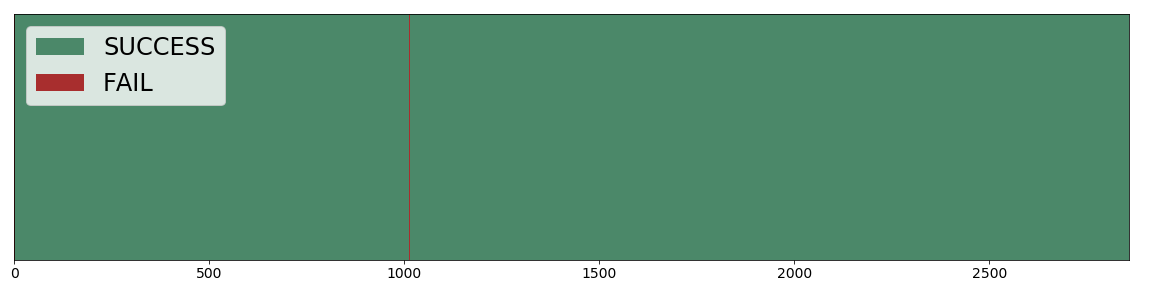
\includegraphics[width=\linewidth]{charts/ClosureHist}
		\caption{Build history of Closure Compiler project}
		\label{fig:closureHist}
	\end{center}
\end{figure}

\section{Apache commons-lang}

\begin{table}[h]
	\caption{Grouped errors in Commons-lang builds}
	\label{table:langErrors}
	\begin{center}
	\begin{tabular}{lr}
		\toprule
		\bf{Error} & \bf{count} \\ 
		\midrule
		There is no POM in this directory & 1,524 \\
		Unmappable character for encoding UTF8	& 110 \\
		error: cannot find symbol in NullComparator.java & 20 \\
		Non-resolvable parent POM & 5 \\
		error: cannot find symbol in UnicodeUnescaper.java & 2 \\
		IDKey is not public in org.apache.commons.lang & 2 \\
		Error: variable options might not have been initialized & 2 \\
		Error: incompatible types & 2 \\
		Others & 6 \\
		\bottomrule
	\end{tabular}
	\end{center}
\end{table}

%\grex{I see some of the errors begin with ``Error: '', others don't. Could we have families of higher-level errors?}

In this project we can observe a consistent build failure starting around the middle of the history (Figure~\ref{fig:langHist}).
In this case, we obtain a failure rate that reaches almost half of the project (46.86\%).
The errors collected for this project are shown in Table~\ref{table:langErrors}.

\begin{figure}[h]
	\begin{center}
		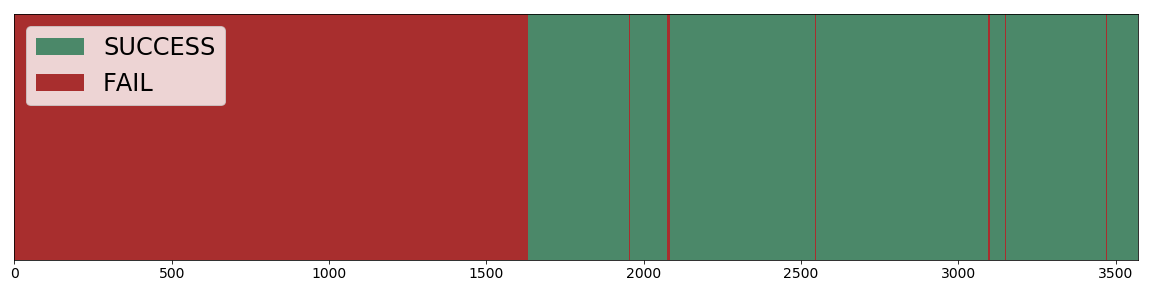
\includegraphics[width=\linewidth]{charts/LangHist}
		\caption{Build history of Apache Commons-lang project}
		\label{fig:langHist}
	\end{center}
\end{figure}

The main error of this project is the absence of the \textit{pom.xml} \emph{config} file, which is used by the maven build system to build the application.
When we looked into this, it was clear that this happened because the build system changed at some point; the project stopped using Ant to start using Maven.

\section{Apache commons-math}

The Math project is a robust one (Figure~\ref{fig:mathHist}), with a low failure rate (20.91\%).
Similar to the commons-lang project, there is a specific commit from which the builds begin to fail.
The errors collected are shown in Table~\ref{table:mathErrors}.

\begin{figure}[h]
	\begin{center}
		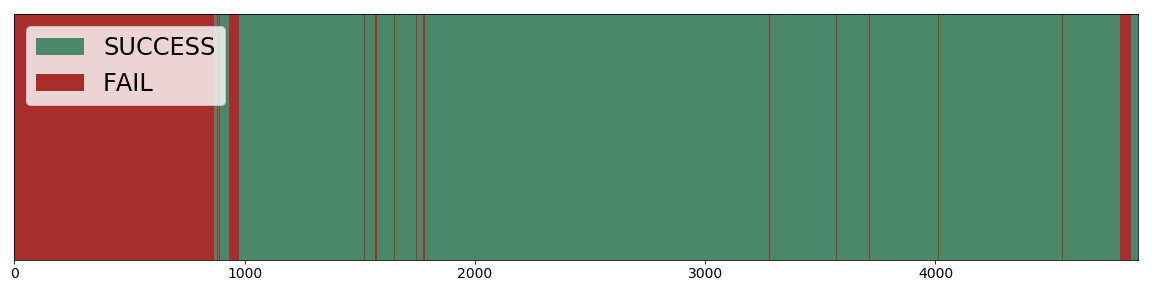
\includegraphics[width=\linewidth]{charts/MathHist}
		\caption{Build history of Apache Commons-math project}
		\label{fig:mathHist}
	\end{center}
\end{figure}


As in the Lang project, the build system for the project was changed, from Ant to Maven, which causes any build to fail in the most recent commits of the project.

\begin{table}[h]
	\caption{Grouped errors in Commons-math builds}
	\label{table:mathErrors}
	\begin{center}
	\begin{tabular}{lr}
		\toprule
		\bf{Error} & \bf{count} \\ 
		\midrule
		Can't read pom.xml: No such file or directory & 866 \\
		Failed to execute goal jacoco-maven-plugin & 52 \\
		Failed to execute goal cobertura-maven-plugin & 43 \\
		Error: cannot find symbol & 28 \\
		Failed to execute goal maven-compiler-plugin & 10 \\
		error: no suitable method found & 4 \\
		error: data has private access in ArrayFieldVector & 2 \\
		error: cannot assign a value to final variable entries & 2 \\
		error: Java name clash, have the same erasure & 2 \\
		error: SparseRealMatrix is not abstract & 2 \\
		error: LUDecompositionImpl is not abstract & 2 \\
		Others & 7 \\
		\bottomrule
	\end{tabular}
	\end{center}
\end{table}

\section{Mockito}

This project shows a very low buildability.
Most of its history commits (see Figure~\ref{fig:mockitoHist}) cannot be built.

\begin{figure}[h]
	\begin{center}
		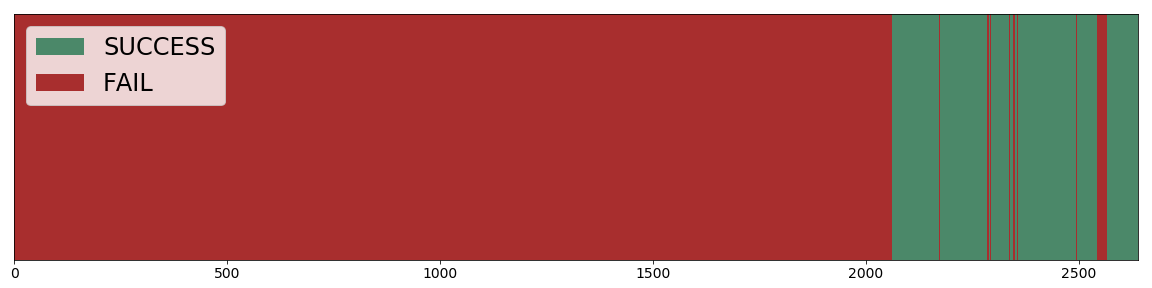
\includegraphics[width=\linewidth]{charts/MockitoHist}
		\caption{Build history of Mockito project}
		\label{fig:mockitoHist}
	\end{center}
\end{figure}

\begin{table}
	\caption{Grouped errors in Mockito builds}
	\label{table:mockitoErrors}
	\begin{center}
	\begin{tabular}{lr}
		\toprule
		\bf{Error} & \bf{count} \\ 
		\midrule
			gradlew: No such file or directory & 1,622 \\
			can't read buildSrc/build.gradle: No such file or directory & 440 \\
			Could not find net.bytebuddy:byte-buddy:0.2.0. & 14 \\
			A problem occurred evaluating script & 9 \\
			Execution failed for task ':jar'. & 6 \\
			Execution failed for task ':compileGroovy'.& 4 \\
			Execution failed for task ':compileJava'. &	3 \\
			unable to resolve class ReleaseNotesServices & 2 \\
			Others & 1 \\
		\bottomrule
	\end{tabular}
	\end{center}
\end{table}

The analysis of errors (Table~\ref{table:mockitoErrors}) shows that the main error found is that the \emph{gradlew} executable does not exist, due to a change in build system from Ant a Gradle.
Another very repeated error is the non-location of the build.gradle file, that was moved at some point to a different folder.


\section{Joda-time}

In this case (see Figure~\ref{fig:timeHist}), we found a high percentage of failures (86.95\%) that, in all cases, are due to a change of the build system, from Ant to Maven.

\begin{figure}[h]
	\begin{center}
		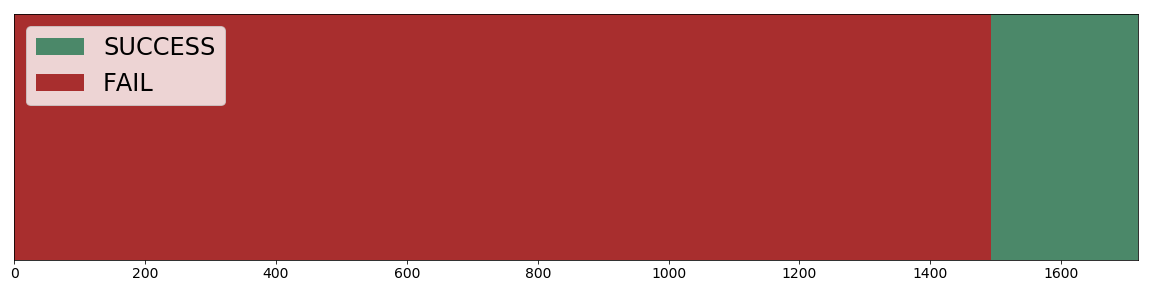
\includegraphics[width=\linewidth]{charts/TimeHist}
		\caption{Build history of Joda-time project}
		\label{fig:timeHist}
	\end{center}
\end{figure}

\section{Spring Framework}

This project is, by far, the one that contains more commits, which gives us a broader vision of how a more complex project behaves.
Just over two-thirds of the project's history (as shown in Figure~\ref{fig:springHist}) cannot be built.
There is a consecutive set of commits where it becomes more buildable.
Finally, in the more recent versions of the project, it is again difficult to find buildable commits.

\begin{figure}[h]
	\begin{center}
		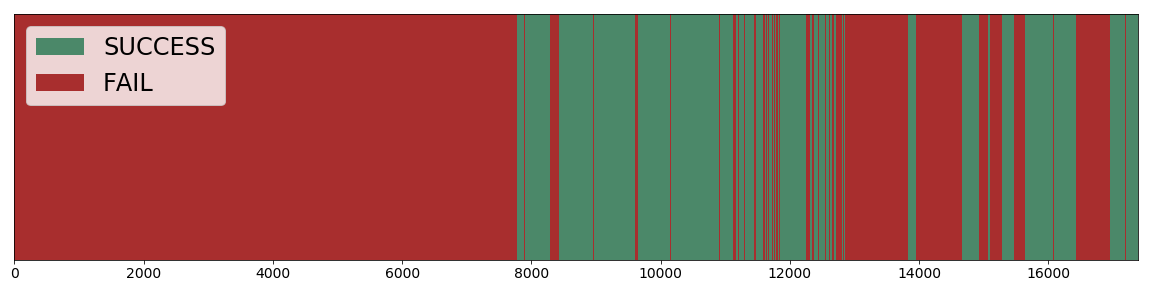
\includegraphics[width=\linewidth]{charts/spring-frameworkHist}
		\caption{Build history of Spring Framework project}
		\label{fig:springHist}
	\end{center}
\end{figure}

\begin{table}
	\caption{Grouped errors in Spring Framework builds}
	\label{table:springErrors}
	\begin{center}
	\begin{tabular}{lr}
		\toprule
		\bf{Error} & \bf{count} \\ 
		\midrule
		gradlew: No such file or directory& 5633  \\
		Cannot allocate memory & 2353  \\
		Invalid byte tag in constant pool & 470   \\
		Could not find group:com.itextpdf & 460   \\
		The import java.util.Arrays cannot be resolved & 398   \\
		error: warnings found and -Werror specified 1 error & 328   \\
		Bad file descriptor & 299   \\
		error: cannot find symbol & 218   \\
		error: incompatible types & 210   \\
		Could not determine which tasks to execute  & 206   \\
		error: unmappable character for encoding ASCII  & 202   \\
		Could not resolve all dependencies for spring-webmvc:optional & 132   \\
		error: constructor (..) cannot be applied to given types & 80 \\
		Execution failed for task ':spring-asm:compileJava'. & 77    \\
		error: constructor (..) cannot be applied to given types & 72    \\
		error: EmbeddedDataSourceProxy is not abstract & 64    \\
		FileNotFoundException & 41    \\
		error: package javafx.application does not exist & 28    \\
		Could not resolve all files for configuration ':classpath'. & 25    \\
		Could not find reactor-net:1.1.0.BUILD-SNAPSHOT. & 19    \\
		Could not find reactor-core:1.0.0.BUILD-SNAPSHOT. & 10    \\
		A problem occurred evaluating root project 'spring' & 9 \\
		error: no suitable method found & 6 \\
		A problem occurred evaluating root project 'spring' & 6     \\
		error: local variable (..) is accessed from within inner class & 3     \\
		error: GenericApplicationContext is not abstract & 3     \\                                                                       
		error: invalid method declaration; return type required & 2  \\
		error: package (..) does not exist & 2 \\    
		Others & 10 \\
		\bottomrule
	\end{tabular}
	\end{center}
\end{table}

As can be seen in Table \ref{table:springErrors}, the number of different errors for this project is far above any other of the studied projects.
The most common error is once again due to a change in the build system, from Ant to Gradle.
Other problems, derived from being a heavy and complex project, are the lack of memory to run the builds and the problem of downloading old or outdated libraries.

\vspace{0.3cm}
\begin{tcolorbox}[fonttitle=\bfseries,title=Answer to RQ1: Can we build all snapshots of a project?,label=rq1,colframe=blue!50!black]
	There are many parts of the history of projects that are not buildable.
	Despite Java being an static typed language, with well-known build systems, four out of six projects have build problems in more than 40\% of their commits.
\end{tcolorbox}











\chapter{Taxonomy of failures}
\label{sec:taxonomy}
Once we analyzed the results for each of the projects, we had a closer look at the different errors and create a taxonomy that could be used for any Java project and answering \textbf{RQ2}.

As we mentioned in the methodology section (See Section \ref{subsec:taxonomy}), we will use the taxonomy development method of Nickerson et al.~\cite{Nickerson2013}. The objective of this section, therefore, will be to classify the errors obtained from the failed builds.

First step in this methodology is to define a meta-characteristic, a starting point to define the characteristics of our taxonomy. Each characteristic should be a logical consequence of the metacharacteristic. In our case, the meta-characteristic will be "\textit{the nature of the fail}". 

The objects that we will use for the development of the taxonomy were the errors obtained in the previous phase (what we called symptoms), a total of 86 errors from the 6 subject proyects. These errors have been randomly divided into 5 groups of 17-18 errors. Five iterations have been carried out using the method, the results of which are shown below:

\begin{enumerate}[\bfseries {I}ter{a}t{i}on 1]
	
	%\vspace{3mm}
	\item For this iteration a \textit{conceptual-to-empirical} approach has been used, using as a starting point a previous taxonomy, \textit{Build Errors: A Case Study}~\cite{Seo:2014:PBE:2568225.2568255}, from which we take the types of errors \textit{Semantic} (Not override a superclass or interface method when use override annotation, incompatible types, not suitable method \dots), \textit{Syntax} (keywords expected, illegal start of expression, statement expected, parsing XML files~\dots) and \textit{Dependency} (can not import this package, could not resolve a library or a version of it \dots), which are common in Java proyects. Since these types do not cover all objects, it is necessary to switch to an empirical approach and add two new types: \textit{Encoding} (using bad encoder for strings) and \textit{Build System} (any problem related to de execution of the build system technology). The taxonomy resulting from this iteration is: \textit{$T_{1}$ = {Type(Build System, Dependency, Encoding, Semantic, Syntax)}}.
	
	\vspace{2mm}
	\item For this iteration a \textit{empirical-to-conceptual} approach has been used. In this iteration, all objects are classified with the current taxonomy, so there is no need to expand it. The taxonomy resulting from this iteration is: \textit{$T_{2}$ = {Type(Build System, Dependency, Encoding, Semantic, Syntax)}}.
	
	\vspace{2mm}
	\item For this iteration a \textit{conceptual-to-empirical} approach has been used. When no new types are detected in last iteration, the use of another dimension of the objects is explored. In the development of an application, we can find that we have made mistakes in the source code, in the configuration or the error is external. This new dimension, the location, could take the following values: Source code, config files or external. Applying this new dimension on the objects of this iteration, all are classified within the domain of the new dimension. No new types arise. The taxonomy resulting from this iteration is: \textit{$T_{3}$ = {Type(Build System, Dependency, Encoding, Semantic, Syntax), Location(Source code, Config files, External) }}.
	
	\vspace{2mm}
	\item For this iteration a \textit{empirical-to-conceptual} approach has been used. From the logs of this iteration, we find that the taxonomy is insufficient and it is necessary to extend it. The type Enviroment (problems in the execution environment) is added. The taxonomy resulting from this iteration is: \textit{$T_{4}$ = {Type(Build System, Dependency, Encoding, Enviroment, Semantic, Syntax), Location(Source code, Config files, External) }}.
	
	\vspace{2mm}
	\item For this iteration a \textit{empirical-to-conceptual} approach has been used. In this iteration, all objects are classified with the current taxonomy, so there is no need to expand it. The taxonomy resulting from this iteration is: \textit{$T_{5}$ = {Type(Build System, Dependency, Encoding, Enviroment, Semantic, Syntax), Location(Source code, Config files, External) }}.
\end{enumerate}          

In figure~\ref{fig:taxonomyTree} we can see the final taxonomy. The classification of the errors made is summarised by project in table \ref{table:taxonomyResults}.

\begin{figure}[h!]
	\begin{center}
		\includegraphics[width=11cm]{img/Taxonomy}
		\caption{Developed taxonomy of software build errors}
		\label{fig:taxonomyTree}
	\end{center}
\end{figure}

\begin{table*}
	\caption{Taxonomy results}
	\label{table:taxonomyResults}
	\centering
	\begin{tabular}{>{\rowmac}r>{\rowmac}r>{\rowmac}r>{\rowmac}r>{\rowmac}r>{\rowmac}r>{\rowmac}r>{\rowmac}r<{\clearrow}}
		\setrow{\bfseries} & CLOSURE & LANG    & MATH    & MOCKITO & SPRING  & TIME     & Average \\
		\toprule
		\setrow{\bfseries}
		Build system & 33.33\% & 91.15\% & 94.41\% & 98.62\% & 61.18\% & 100.00\% & 79.78\%        \\
		\midrule
		Config Files & 0.00\%  & 0.06\%  & 0.00\%  & 21.42\% & 1.93\%  & 0.00\%   & 3.90\%         \\
		External     & 33.33\% & 91.09\% & 94.41\% & 77.20\% & 59.25\% & 100.00\% & 75.88\%        \\
		\midrule
		\setrow{\bfseries}
		Dependency   & 33.33\% & 0.30\%  & 0.00\%  & 0.95\%  & 9.55\%  & 0.00\%   & 7.36\%         \\
		\midrule
		Config Files & 0.00\%  & 0.30\%  & 0.00\%  & 0.67\%  & 5.69\%  & 0.00\%   & 1.11\%         \\
		External     & 0.00\%  & 0.00\%  & 0.00\%  & 0.00\%  & 0.36\%  & 0.00\%   & 0.06\%         \\
		Source Code  & 33.33\% & 0.00\%  & 0.00\%  & 0.29\%  & 3.50\%  & 0.00\%   & 6.19\%         \\
		\midrule
		\setrow{\bfseries}
		Encoding     & 0.00\%  & 6.58\%  & 0.00\%  & 0.00\%  & 1.78\%  & 0.00\%   & 1.39\%         \\
		\midrule
		Source Code  & 0.00\%  & 6.58\%  & 0.00\%  & 0.00\%  & 1.78\%  & 0.00\%   & 1.39\%         \\
		\midrule
		\setrow{\bfseries}
		Enviroment   & 0.00\%  & 0.00\%  & 0.00\%  & 0.00\%  & 20.70\% & 0.00\%   & 3.45\%        \\
		\midrule
		External     & 0.00\%  & 0.00\%  & 0.00\%  & 0.00\%  & 20.70\% & 0.00\%   & 3.45\%        \\
		\midrule
		\setrow{\bfseries}
		Semantic     & 33.33\% & 1.85\%  & 5.59\%  & 0.43\%  & 6.78\%  & 0.00\%   & 8.00\%         \\
		\midrule
		Source Code  & 33.33\% & 1.85\%  & 5.59\%  & 0.43\%  & 6.78\%  & 0.00\%   & 8.00\%         \\
		\midrule 
		\setrow{\bfseries}
		Syntax       & 0.00\%  & 0.12\%  & 0.00\%  & 0.00\%  & 0.02\%  & 0.00\%   & 0.02\%         \\
		\midrule
		Config Files & 0.00\%  & 0.06\%  & 0.00\%  & 0.00\%  & 0.00\%  & 0.00\%   & 0.01\%         \\
		Source Code  & 0.00\%  & 0.06\%  & 0.00\%  & 0.00\%  & 0.02\%  & 0.00\%   & 0.02\%        
	\end{tabular}
\end{table*}

\vspace{0.3cm}
\begin{tcolorbox}[fonttitle=\bfseries,title=Answer to RQ2: What are the most common problems that cause
	snapshot build fail?,label=rq2,colframe=blue!50!black]
	Considering the taxonomy made and the errors classified in it, we can conclude that the most common errors we find when building the snapshot of a Java project are due to the Build System (79.78\%), to the semantics of the language (8.00\%) and to the dependencies of the project (7.36\%). Other less common errors are related to the environment (3.45\%), encoding (1.39\%) and syntax (0.02\%).
\end{tcolorbox}


\chapter{Discussion}
\label{sec:discussion}
This section discusses implications of the experimental results, the observations from our study on buildability and the proposed taxonomy, followed by an approximation of mitigation measures. In addition, it discusses limitations and threats to validity.

\section{Implications of experimental results}

First, we expected the projects to have a stable build history (all of them are Open Source libraries), with some points in the past where the project could not be built. This idea has only materialized in the Closure project. In the rest of the projects we have found a common problem, a change in the build system of the project, which considerably reduces the number of buildable commits. The main disadvantage of pre-setting the construction system and assuming that it will not vary significantly affects the study, but at the same time gives us valuable information about the evolution of the projects and how we must adapt.

Running the experimentation required a significant investment of time and resources. It was necessary to run the experiment on isolated machines (one per project) that were running for several days sequentially executing the builds of each project. Some measures to mitigate the amount of time required were the elimination of tasks at build process that did not directly affected the project, such as the generation of automatic documentation or the execution of tests, which was not considered within the scope of the experiment. In some projects, as in the case of Spring Framework, there was the problem of Maven Central (from where dependencies are downloaded) banning the IP of the machine as a result of an abuse of the API, that externally prevented the correct build of the project, having to limit the number of builds per time to avoid it.

\section{Implications of proposed taxonomy}

The taxonomy developed in this work proposes a high-level classification easily extensible that collects the types of errors and their location in the project. The taxonomy was intended to be an answer to RQ2, but we found that this is only one dimension within the most exhaustive classification that can be carried out. We introduce the dimension of the location of the error (in which place of the project it occurs -- or if it occurs outside of it-- ). Other dimensions not included but possible could be the involvement of the developer (complex in some cases due to the lack of knowledge of the development phase) in the error or the difficulty of its solution (it can be subjective).

Most of the problems we find in the construction of a project are not affected by the compilability of the project, so they would be extendable to the scope of dynamic languages

%Providing a categorization of errors empirically is not easy. We must leave any preconceived ideas of what the problems will be like to stick only to the results. Initially, we found all built problems unclassified, we only knew where were they localized in the history of commits. By grouping together problems related to consecutive commits we found that usually the build failures were produced by the same problem. Once grouped, it was enough to choose a failed build, check its log and extract the pattern that identified it to apply it again to all the failed builds. This process was repeated until there was no unclassified failed builds. The patterns had to be generic enough to be able to capture different variants of the same error, but in some cases it was necessary to particularize the error in order to get the specific classification.

%Common patterns were found for the different Java projects, independent of the build system used, such as

%\begin{lstlisting}
%	error: (.+)\n(.+)
%\end{lstlisting}

%which classifies the errors derived from the compilation of Java code and in turn allows subcategories based on their variants, for example

%\begin{lstlisting}
%	error: incompatible types
%\end{lstlisting}

%These cases strengthen our choice of Java as a technology on which to investigate buildability: the structured logs provided by the compiler and build systems allowed us to make a simple and automated tracking of errors.

\section{Mitigation measures}

While we were doing the taxonomy, we realize that some of the problems we encountered could be easily solved to achieve a successful build and others were more complicated or unfeasible.

Some generic solutions, that requires changes in the configuration or in the command launched by the project but not in the source code itself, follows:

\begin{itemize}
	\item \textbf{Build system change} Detect which technology is being used to build the project to use the most convenient one in each case (search pom.xml for Maven, build.xml for Ant, and so on)
	\item \textbf{Encoding problem} If it does not exist, add the property encoding in the project configuration file.
	\item \textbf{Dependency problem} If a dependency is a SNAPSHOT, look for the compatible version that is stable and recoverable from the dependency repository. Replace this dependency with the stable one in the configuration before executing the build.
	\item \textbf{Environment problem} Check the resource requirements of the project.
\end{itemize}

For the following problems, the solution is usually not trivial or cannot easily be automated:

\begin{itemize}
	\item \textbf{Java compilation issue: Syntax and semantic} Requires modification of the source code of the project.
	\item \textbf{Build configuration issues} Requires a deep knowledge of how the project is built.
\end{itemize}

These problems are usually specific code errors that do not affect too many versions, because the developers often correct them quickly.

\section{Limitations and Threats to Validity}

The validity of our work is described in terms of the four main threats to validity in empirical software engineering research: construct, internal and external validity~\cite{Wohlin2012} (excluding statistical conclusion validity that does not apply to our problem).

% Construct validity: Does the treatment correspond to the actual cause we are interested in? Does the outcome correspond to the effect we are interested in?

\textbf{Construct validity} 
The results of the analysis corresponding to the RQ1 are affected essentially by the construction system of the project, so that a large number of fail builds of the projects may be hiding other causes of errors. We believe that an undocumented change in the way the project is built is a cause of error in itself.

%\hspace{5px}

% Internal validity: Did the treatment/change we introduced cause the effect on the outcome? Can other factors also have had an effect?

\textbf{Internal validity} Threats to internal validity relate to the experimenter; taxonomy has been made from empirical data (the logs of the failure builds) under the interpretation of a single researcher who performed the analysis. On the other hand, a well-documented taxonomy methodology has been used along with conceptual approaches in some of the iterations, specifically using in one of them the previous knowledge of taxonomy of errors in Java projects from another work.

%\hspace{5px}

% External validity, Transferability Is the cause and effect relationship we have shown valid in other situations? Can we generalize our results? Do the results apply in other contexts?

%\noindent
\textbf{External validity} A general threat to external validity is the representativeness of the selected subjects. In this study we use open source projects, which could not be representative of other software projects. However, we think we took this issue into consideration by including the Spring Framework project, which is a huge project heavily used in the industry, which is a good representative of a big project. 

% Conclusion validity: Does the treatment/change we introduced have a statistically significant effect on the outcome we measure?

%\textbf{Conclusion validity}  

%\grex{Include a sentence about construct and conclusion validity (related to how sure the conclusions reached in regards to the relationships in our data are reasonable.)}








\chapter{Conclusions and future Work}
\label{sec:conclusions}
In this work, we investigate the buildability of all snapshots of a software project. We present the buildability study of six real open source projects and create an extensible taxonomy of build failures based on the empirical results found. We propose as well a tool to easy reproduce the experiment in any project to extend this investigation.


Analyzing build errors we noted that high percentage of them are caused by external build system errors. A deeper inspection in this category shows us that the main error is a change at build system technology along the history of the project. We can see an example of this error in Mockito project. A change of build system from Ant to Gradle is reported as a build error in 60\% of its commits with the symptom \textit{gradlew: No such file or directory}.

With the proposed procedure we build all snapshots of a project using the build system indicated in the official documentation.
But if the build system change along the history, is reasonable that build fails when it changes.
%If we choose the correct building system for each snapshot, we would be able to improve the buildability of the project history. 
If we analyze the errors not related with build system change, we can estimate that more than 82\% of the project history would be buildable.

We believe that this study could allow and facilitate further research on related topics, such as error localization, where the identification of success builds would help us greatly.  

\bibliographystyle{abbrv}
\bibliography{bibliography} 

\end{document}


